% !TEX root = quickstep.tex

\section{Storage Manager} \label{storage-manager}

The \Quickstep\ storage manager~\cite{ChasseurP13} is based on a  block-based architecture, which we describe next. The storage manager allows a variety of physical data organizations to coexist within the same database, and even within the same table. We briefly outline the block-based storage next.

%(See~\cite{ChasseurP13} for a more detailed description.) %We have chosen this highly-flexible and extensible design for physical storage based on empirical experiments that show that the performance of core data-intensive relational operations like selection and projection can be very sensitive to the layout of data in memory, and
%This design leverages the insight that there is no single ``one size fits all'' storage organization %that achieves good performance
%for all workloads~\cite{ChasseurP13}.
\subsection{Block-Structured Storage} \label{block-structure}
Storage for a particular table in \Quickstep\ is divided into many blocks with possibly different layouts, with individual tuples wholly contained in a single block. Blocks of different sizes are supported, and the default block size is 2 megabytes. On systems that support large virtual-memory pages, \Quickstep\ constrains block sizes to be an exact multiple of the hardware large-page size (e.g. 2 megabytes on x86-64) so that it can allocate buffer pool memory using large pages and make more efficient use of processor TLB entries.

Internally, a block consists of a small \textit{metadata header} (the block's self-description), a single \textit{tuple-storage sub-block} and any number of \textit{index sub-blocks}, all packed in the block's contiguous memory space. There are multiple implementations of both types of sub-blocks, and the API for sub-blocks is generic and extensible, making it easy to add more sub-block types in the future. Both row-stores and column-store formats are supported, and orthogonally these stores can be compressed. See~\cite{storage-blog-post} for additional details about the block layouts.


\subsection{Compression} \label{sec-compression}
Both row store and column store tuple-storage sub-blocks may optionally be used with compression. \Quickstep\ supports two type-specific order-preserving compression schemes: (1) simple ordered dictionary compression for all data types, and (2) leading zeroes truncation for numeric data types. In addition, \Quickstep\ automatically chooses the most efficient compression for each attribute on a per-block basis.

Dictionary compression converts native column values into short integer codes that compare in the same order as the original values. Depending on the cardinality of values in a particular column within a particular block, such codes may require considerably less storage space than the original values. In a row store, compressed attributes require only 1, 2, or 4 bytes in a single tuple slot. In a column store, an entire column stripe consists only of tightly-packed compressed codes.  We note
that in the column-store case, we could more aggressively pack codes without ``rounding up'' to the nearest byte, but our experiments have indicated that the more complicated process of reconstructing codes that span across multiple words slows down scans overall when this technique is used. Thus, we currently pack codes at 1, 2, and 4 byte boundaries.


%Quickstep supports type-specific order-preserving compression schemes.
%For numeric data types, Quickstep suppresses leading zeroes. For other data types, ordered dictionary compression is used. The dictionaries are constructed on a per-block basis and are contained within the block.

%Dictionary compression converts native column values into short integer codes that compare in the same order as the original values. Depending on the cardinality of values in a particular column within a particular block, such codes may require considerably less storage space than the original values. In a row store, compressed attributes require only 1, 2, or 4 bytes in a single tuple slot. In a column store, an entire column stripe consists only of tightly-packed compressed codes.  We note that in the column-store case, we could more aggressively pack codes without ``rounding up'' to the nearest byte, but our experiments have indicated that the more complicated process of reconstructing codes that span across multiple words slows down scans overall when this technique is used. Thus, we currently pack codes at 1, 2 and 4 byte boundaries.

%Because Quickstep uses order-preserving compression, comparison predicates can directly be evaluated on the compressed codes (without decompressing). This means that we may use considerably less memory bandwidth and cache space when scanning a compressed column (especially with a column store). Additionally, comparing integer codes requires only a simple single-cycle CPU instruction, while comparing more complex uncompressed data types (e.g. strings) can be more CPU-intensive.

%On the other hand, compression introduces an additional level of indirection when native values have to be accessed by looking them up in a dictionary (e.g. when doing projection). Thus, whether compression is valuable for a particular query  is dependent on the query selectivity. %Our observations on the performance trade-offs associated with compression are outlined in~\cite{ChasseurP13}.



% When a tuple is inserted into a block, all column values are stored in the tuple-storage sub-block, and any applicable index sub-blocks are updated (index sub-blocks always refer to tuples in the same block, and thus indices are self-contained at the block level and always colocated with data).

%\subsection{Micro-Optimization} \label{sec:micro-opt}
%Each \Quickstep\ block can be considered to be a mini self-contained database exposing an API consisting of a set of logical and relational operations. These operations include selection (predicate evaluation), projection (materializing output to other in-memory blocks), tuple insertion (both tuple-at-a-time and batch-oriented), in-place updates and deletes (with optional predicates), and sorting. The actual implementation of these operations may be different depending on what sub-blocks are present in a particular block, and each block decides for itself, based on its own internal organization, how to execute a particular call efficiently.

%In fact, a block contains a micro-optimizer that, at run-time, evaluates the cost of performing a given operation using each of its sub-blocks, and chooses the lowest-cost physical plan. Thus, the relational operators need not concern themselves with the internal structure of different storage blocks, and can instead use the common block API. For instance, a single selection predicate may be satisfied using a scan of the tuple-storage sub-block or by using any of the available index sub-blocks. A complex predicate may use different plans for different predicates, and the results are combined using bit-wise operations on bit-vectors of matches. (A ``filter'' bit-vector can also be passed when invoking the operation, which can then be used to skip over or short-circuit the evaluation of some predicates within a conjunction or disjunction that has already been decided for some tuples).

%The block-based storage model grants the system the flexibility to make different layout and indexing decisions for different parts of the same relation, depending on their access patterns. However, this diversity poses a challenge to traditional database engines that make access path decisions during query optimization. In principle, the micro-optimization framework in \Quickstep\ allows execution plans to adapt to run-time conditions such as data and query characteristics, without increasing query optimization complexity. Currently, this micro-optimizer simply employs a pre-defined order of preference for different applicable access paths, but we plan to add basic statistics and selectivity estimation in the future.

\subsection{Template Metaprogramming}
\label{vectorization}

As noted above, Quickstep supports a variety of data layouts (row vs. column store, and with and without compression). Each operator algorithm (e.g. scan, select, hash-based aggregate, hash-based join, nested loops join) must work with \textit{each} data layout. From a software development perspective, the complexity of the software development for each point in this design space can be quite high. A naive way to manage this complexity is to use inheritance and dynamic dispatch. However, the run-time overhead of such indirection can have disastrous impact on query performance. %Most modern systems~\cite{Neumann11, SparkSQL} now use dynamic code generation to address this concern.

To address this problem, Quickstep uses a template metaprogramming approach to allow efficient access to data in the blocks. This approach is inspired by the principle of zero-cost abstractions exemplified by the design of the C++ standard template library (STL), %In the STL,
in which the implementations of containers (such as vectors and maps) and algorithms (like find and sort) are separated from each other.
%The crucial abstraction that enables this separation is the notion of iterators, which allow containers to expose common data access patterns (hiding implementation details) and algorithms to be implemented against the iterator interface (rather than containers directly).

\Quickstep\ has an analogous design wherein access to data in a sub-block is made via a \texttt{ValueAccessor} in combination with a generic functor (usually a short lambda function) that implements the evaluation of some expression or the execution of some operator algorithm. The various ValueAccessors and functors have been designed so that the compiler can easily inline calls and (statically) generate compact and efficient inner loops for expression and operator evaluation described in more detail below in Section~\ref{ssec:expression-eval}. Such loops are also amenable to prefetching and SIMD auto-vectorization by the compiler, and potentially (in the future) mappable to data parallel constructs in new hardware. (We acknowledge that there is a complementary role for run-time code generation.) We describe the use of this technique for expression evaluation next.

%Projection may involve evaluating arbitrary expressions on column values in the projection list.
%Note that the use of template metaprogramming is relatively easy in a language like C++, which is the programming language for \Quickstep. In contrast to run-time code generation techniques there is no additional run-time cost, but there is an increase in the (one-time) compilation cost and the size of the compiled binary.

\begin{figure}
\centering
   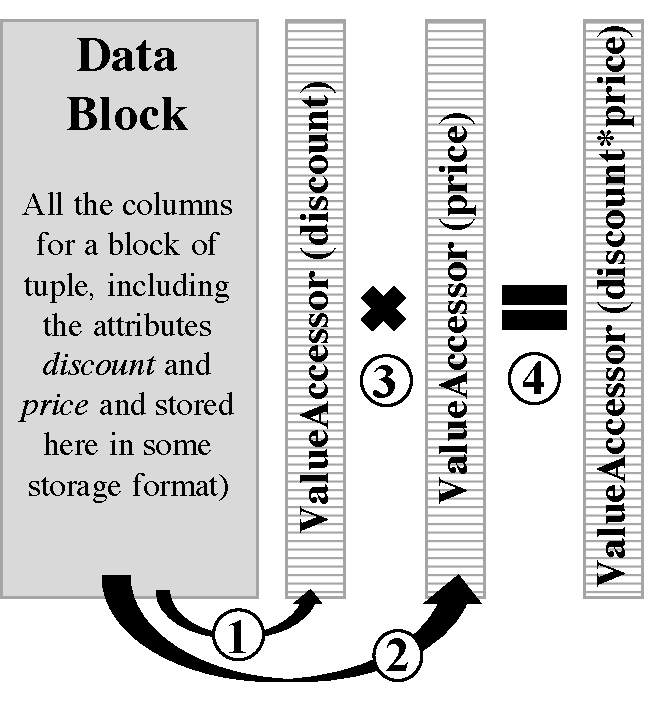
\includegraphics[width=0.25\textheight]{system/figures/VA.pdf}
   \caption{\textbf{Evaluation of the expression \texttt{discount*price}.}}
   \label{fig-template-VA}
\end{figure}


\subsubsection{Expression Evaluation}\label{ssec:expression-eval}
The \texttt{ValueAccessor}s (VAs) play a crucial role in efficient evaluation of expressions (e.g. \texttt{discount*price}). Figure~\ref{fig-template-VA} illustrates how VAs work using as example an expression that is the product of two attributes. There are  various compile time optimizations that control the code that is generated for VAs. When using the ``Basic'' optimization, the VA code makes a physical copy of the attributes that are referenced in the expression. These are steps 1 and 2 in Figure~\ref{fig-template-VA}. The vector of the two attributes are then multiplied (step 3 in the figure) using a loop unrolled by the compiler (possibly generating SIMD instructions).  The output of the expression is another VA object, from which (efficient) copies can be made to the final destination (likely a sub-block in a result block).

When using the ``Selection'' optimization level, the code that is generated for the VAs uses an indirection to the attributes (regardless of the storage format in the block). Thus, in steps 1 and 2 in Figure~\ref{fig-template-VA}, the resulting VA ``vectors'' contain pointers to the actual attributes. These pointers are dereferenced as needed in step 3. With the Selection optimization, copies are avoided, and if the columns are in a columnar store format the VAs are further compacted to simply point to the start of the ``vector'' in the actual storage block.

To understand the impact of the template metaprogramming  approach we compared the code generated by the template metaprogamming (i.e. VA) approach with a standalone program that uses dynamic dispatch to access the attributes. With the dynamic dispatch option, a traditional \texttt{getNext()} interface is used to access the attributes in a uniform way regardless of the underlying storage format. For this comparison, we created a table with two integer attributes, set the table cardinality to 100 million tuples, and stored the data in a columnar store format. Then, we evaluated an expression that added both the integer attributes (on the same 2 socket system described in Section~\ref{evaluation}). The resulting code using the Selection optimization is 3X faster compared to the virtual function approach when using a single thread (when the computation is compute-bound, and drops to 2X when using all the (20) hardware threads when the computation is more memory-bound.

%As noted above since Quickstep supports multiple storage formats, to evaluate an expression, we need an interface to access the attribute values in a storage block in a uniform way so that the caller function does not have to worry about the underlying storage format (to keep the code complexity down).  A naive design for such an interface is an iterator that has a \texttt{getNext()} virtual call (i.e. dynamic dispatch).
%Each storage format could implement the \texttt{getNext()} interface based on its physical layout.
%But, the cost of such virtual calls can be high (3X as noted below).



%\textcolor{blue}{The solution to this challenge in \Quickstep\ is through the template metaprogramming technique described above. \Quickstep\ has a system of code templates to access column values of a particular type in a particular kind of tuple-storage sub-block. Thus, scalar expressions compile down to tight, vectorizable loops without in-loop branching or indirection that materialize the result of an expression for all the tuples in a block. %(optionally filtered by a bit-vector of predicate matches) in one pass. Note that this system of template-based vectorized expression evaluation is also used when evaluating arbitrary expressions that are nested within predicates. }
%

%\textcolor{blue}{\Quickstep\ use the ValueAccessor to evaluate expressions efficiently. There are  various compile time optimization that relate to how the ValueAccessor is constructed. When using the ``Basic'' optimization, the ValueAccessor code creates a physical copy of the attributes that are  referenced in the expression. These are steps 1 and 2 in Figure~\ref{fig-template-VA}. The vector of the two attributes (discount and price) are then added (step 3 in the figure) using a loop that is automatically unrolled by the compiler (possibly generating SIMD instructions).  The output of the expression is another ValueAccessor object, from which (efficient) copies can be made to the final destination (likely as sub-block in a result block).}



%%These intermediate column results are stitched together and bulk-inserted into another in-memory block. In the common case where the projection list only copies attribute values as-is from the input, we skip the expression evaluation and use the same template system to directly bulk-copy tuple data from one block into another.

%Other operations like building and probing hash tables for hash joins, aggregation over a block (both simple and hash-based), and sorting also use the code template system so that data-intensive tuple-by-tuple ``inner loops'' are as simple as possible and avoid branching or indirection to deal with different data types and different storage layouts.

%{\color{blue}
%
%Listing \ref{lst:copy-elision-basic} shows a simplified code fragment for scalar expression evaluation on two columns with copy elision level {\bf Basic}.
%
%With copy elision Basic, we first materialize the columns from their underlying storage into compact column vectors (\texttt{CV}). Then we specialize on the columns' types to generate tight loops where inlined evaluation gets performed.
%
%Note that the main reason to materialize the columns is to reorganize the memory layout -- conforming to a ``protocol" -- that the columns can be interpreted as a compact C array. So that C++ compilers can generate efficient code, and SIMD intrinsics can be utilized.
%
%\lstinputlisting[language=C++,basicstyle=\ttfamily\scriptsize,
%                   label=lst:copy-elision-basic,
%                   caption=Copy elision level: Basic]{pictures/copy-elision-code-basic.cpp}
%
%Listing \ref{lst:copy-elision-selection} shows copy elision level {\bf Selection}.
%With this copy elision level, the columns are not materialized. Instead, we implement the value accessors to conform to a protocol (or ``concept", in C++ terminology) that is analogous to C++ \emph{BidirectionalIterator}. By specializing on the value accessors, we achieve \emph{static polymorphism} where the underlying storage can be accessed directly with zero overhead. And the compiler has sufficient compile-time information to generate tight loops with inlined evaluation.
%
%\lstinputlisting[language=C++,
%                   basicstyle=\ttfamily\scriptsize,
%                   label=lst:copy-elision-selection,
%                   caption=Copy elision level: Selection]{pictures/copy-elision-code-selection.cpp}

\subsection{Holistic Memory Management}
\label{unified-buffer-manager}
The \Quickstep\ storage manager maintains a \textit{buffer pool} of memory that is used to create blocks, and to load them from persistent storage on-demand. Large allocations of unstructured memory are also made from this buffer pool, and are used for shared run-time data structures like hash tables for joins and aggregation operations. These large allocations for run-time data structures are called \textit{blobs}. The buffer pool is organized as a collection of slots, and the slots in the buffer pool (either blocks or  blobs) are treated like a larger-sized version of page slots in a conventional DBMS buffer pool.

We note that in \Quickstep\ \textit{all} memory for caching base data, temporary tables, and run-time data structures is allocated and managed by the buffer pool manager. This holistic view of memory management implies that the user does not have to worry about how to partition memory for these different components. The buffer pool employs an eviction policy to determine the pages to cache in memory. \Quickstep\ has a mechanism where different ``pluggable'' eviction policies can be activated to choose how and when blocks are evicted from memory, and (if necessary) written back to persistent storage if the page is ``dirty.'' The default eviction policy is LRU-2~\cite{lru-k}. %, but implementation also exist for ``random'' policy and LRU-k with arbitrary k. %, and our pluggable eviction policy system allows implementing other strategies easily in the future.

Data from the storage manager can be persisted through a file manager abstraction that currently supports the Linux file system (default), and also HDFS~\cite{hdfs}. %At this point, we only have a simple database-level locking scheme with just read and write locks.

%\subsection{Block-Structured Storage} \label{block-structure}
%Internally, a block consists of a small metadata header (the block's self-description), a single \textit{tuple-storage sub-block} and any number of \textit{index sub-blocks}, all packed in the block's contiguous memory space. There are multiple implementations of both types of sub-blocks available in \Quickstep\ (as described below), and the API for sub-blocks is generic and extensible, making it easy to add more sub-block types in the future. When a tuple is inserted into a block, all column values are stored in the tuple-storage sub-block, and any applicable index sub-blocks are updated (index sub-blocks always refer to tuples in the same block, and thus indices are self-contained at the block level and always colocated with data).



%\subsection{Tuple Stores} \label{tuple-stores}
%\Quickstep\ currently implements both row store and column store layouts for \textit{tuple-storage sub-blocks}.
%, although other formats (e.g. PAX~\cite{AilamakiDHS01}) are also possible.
%(A detailed analysis of layout options is available in~\cite{ChasseurP13}.)

%\subsubsection{Row Stores}
%Row stores come in two flavors. The first is a ``split'' row-store that uses a conventional slotted-page layout with storage for fixed length attributes growing from one end of the sub-block memory, and storage for variable-length attributes growing from the other end.  The second variety of row-store is a ``packed'' row store which is simply a packed row-major array of fixed-length values, and can not be used with relations that have variable-length attributes.
%All intermediate relations are materialized in row store format.

%\subsubsection{Column Stores}
%A column store tuple-storage sub-block divides sub-block memory into contiguous stripes, one for each column, and stores column values packed within the individual stripes. A column store may optionally be kept sorted on the values of one column.

%\subsubsection{Compression}
%Both row store and column store tuple-storage sub-blocks may optionally be used with compression. \Quickstep\ supports type-specific order-preserving compression schemes. For numeric data types, we suppress leading zeroes. For other data types, we use simple ordered dictionary compression. The dictionaries are constructed on a per-block basis and are contained within the block.

%Dictionary compression converts native column values into short integer codes that compare in the same order as the original values. Depending on the cardinality of values in a particular column within a particular block, such codes may require considerably less storage space than the original values. In a row store, compressed attributes require only 1, 2, or 4 bytes in a single tuple slot. In a column store, an entire column stripe consists only of tightly-packed compressed codes.  We note that in the column-store case, we could more aggressively pack codes without ``rounding up'' to the nearest byte, but our experiments have indicated that the more complicated process of reconstructing codes that span across multiple words slows down scans overall when this technique is used. Thus, we currently pack codes at 1, 2 and 4 byte boundaries.

%Because our implementation of dictionary compression is order-preserving, we can evaluate comparison predicates directly on the compressed codes without decompressing. This means that we may use considerably less memory bandwidth and cache space when scanning a compressed column (especially with a column store). Additionally, comparing integer codes requires only a simple single-cycle CPU instruction, while comparing more complex uncompressed data types (e.g. strings) can be more CPU-intensive.

%On the other hand, compression introduces an additional level of indirection when native values have to be accessed by looking them up in a dictionary (e.g. when doing projection). Thus, whether compression is valuable for a particular query  is dependent on the query selectivity. %Our observations on the performance trade-offs associated with compression are outlined in~\cite{ChasseurP13}.

%\subsection{Indices} \label{indices}
%\Quickstep\ currently implements cache-efficient B+Trees using the CSB+-Tree~\cite{csbtree} method. Small  materialized aggregates (SMAs)~\cite{sma} are also implemented. The SMA component computes minimum, maximum and count aggregates, which are materialized within each block.
%Code for index subblocks that use BitWeaving/H and BitWeaving/V~\cite{bitweaving} have also been implemented. But, it turns out that due to a patent on these techniques, that code could not be contributed to the code base as the patent conflicts with the ASF license. So, we do not discuss indexing further in this paper. For simplicity, in the experiments we simply turn off \textit{all} indexing in \Quickstep.

%All index sub-blocks support the same interface allowing parts of a predicate tree to be evaluated using different sub-blocks, with a bit-vector of matching tuple positions as the common representation for predicate matches. This generic index interface also allows for extensibility whereby new indexing methods can be added.

% Small materialized aggregates (SMAs)~\cite{sma} are also supported.

%\subsubsection{CSB+-Tree} \label{csb-trees}
%The CSB+-Tree (cache-sensitive B+-Tree)~\cite{csbtree} is a modification of the classic B+-Tree, and is designed to achieve good performance in main-memory.
%Nodes in a CSB+-Tree are physically aligned with cache lines, and are allocated in contiguous ``node groups'' so that scanning across sibling nodes has a linear prefetching-friendly memory access pattern. The CSB+-Trees are generally useful for highly-selective lookup queries~\cite{ChasseurP13}.

%\subsubsection{BitWeaving} \label{bitweaving}

%BitWeaving/H and BitWeaving/V are bit-based indexing methods~\cite{bitweaving}, that aim to exploit the bit-level parallelism in the ALUs of modern CPUs (they can also be used with SIMD and GPUs, but in this paper we only use them on the scalar ALUs).  Both are dictionary-based ordered compression techniques. Briefly, BitWeaving/H (horizontal) improves on standard bit-packing for compressed codes by adding a ``padding bit'' next to each code packed into a word (using the technique proposed in~\cite{Lamport75}). Then, it uses a sequence of bitwise operations on the codes in a word that sets the value of the padding bit to 1 or 0 depending on whether a comparison condition matches for the respective code. Codes are organized into groups of words so that a word-long bit-vector of matches can be efficiently constructed by masking and shifting the padding bits.

%BitWeaving/V (vertical) decomposes the bits of a particular code vertically, packing the most-significant bits of several codes together into one word, the second-most-significant bits into the next word, and so on. Comparisons are evaluated bit-by-bit on all the codes in parallel (e.g. on 64 codes in parallel on a typical CPU with 64-bit word size, or 128-512 codes when using SIMD registers). Our implementation includes an ``early pruning'' technique~\cite{bitweaving} to skip over some words containing less-significant bits when a particular comparison can be totally decided for a group of codes by only looking at some of the most-significant bits. The probability of early-pruning is increased when a filter from some other part of a conjunctive predicate is available. %Experimental evaluation of BitWeaving techniques has shown that, for typical code lengths, the average number of CPU cycles/tuple required to evaluate a scan predicate is less than 1, achieving true intra-cycle parallelism~\cite{bitweaving}.
